\documentclass[12pt]{article}

\usepackage{sbc-template}
\usepackage[T1]{fontenc}
\usepackage[utf8]{inputenc}
% Portugues quando o pacote existir (Overleaf/TeX Live completo); senao, fallback.
\IfFileExists{brazil.ldf}{\usepackage[english,brazil]{babel}}{%
  \usepackage[english]{babel}%
  \addto\captionsenglish{\renewcommand{\tablename}{Tabela}%
    \renewcommand{\figurename}{Figura}\renewcommand{\refname}{Referências}}}
\usepackage{graphicx}
\usepackage{booktabs}
\usepackage{url}
\usepackage{microtype}
\usepackage{tikz}
\usetikzlibrary{arrows.meta,positioning}

\sloppy

\title{Adaptação de um Modelo Visão-Linguagem Pequeno para Legendagem
Técnica de Imagens Portuárias em Português}

\author{Alan Soares, Daniel Santos, Lucas Lopes}
\address{Instituto de Computação -- Universidade Federal da Bahia (UFBA)\\
  Salvador -- BA -- Brasil}
\email{alan.soares@ufba.br, daniel.lopes.santoss@gmail.com, gglucas811@gmail.com}

\begin{document}
\maketitle

\begin{abstract}
We evaluate whether a 2B-parameter vision-language model (Qwen3-VL-2B) can be
adapted, with 68 training images, to write technical port captions in
Brazilian Portuguese. Five variants (zero-shot, connector pre-training, full
fine-tuning, LoRA, QLoRA) are compared with a large API model (Gemini Flash).
LoRA and QLoRA raise CIDEr from 0.12 to 0.53, beat full fine-tuning with
15$\times$ fewer trainable parameters and reach 87\% (ROUGE-L) and 95\%
(BERTScore) of the large model. CLIPScore ranks the variants in reverse.
\end{abstract}

\begin{resumo}
Avaliamos se um modelo visão-linguagem de 2 bilhões de parâmetros
(Qwen3-VL-2B) pode ser adaptado, com 68 imagens de treino, para gerar
legendas técnicas portuárias em português. Cinco variantes (zero-shot,
pré-treino do conector, fine-tuning completo, LoRA e QLoRA) são comparadas a
um modelo grande via API (Gemini Flash). LoRA e QLoRA elevam o CIDEr de 0,12
para 0,53, superam o fine-tuning completo com 15$\times$ menos parâmetros
treináveis e atingem 87\% (ROUGE-L) e 95\% (BERTScore) do modelo grande.
O CLIPScore inverte a ordem das variantes.
\end{resumo}

\section{Introdução}

Portos inteligentes (\textit{smart ports}) integram sensores, câmeras e
sistemas de informação para dar visibilidade às operações
\cite{molavi2020,yang2018}. Boa parte desses dados é visual, e a legendagem
automática de imagens (\textit{image captioning}) os transforma em texto
para indexação, relatórios, acessibilidade e agentes baseados em LLM. VLMs
grandes fazem isso bem, mas exigem APIs pagas, enviam as imagens a terceiros
e conhecem pouco o jargão portuário em português (portêiner, transtêiner,
\textit{reach stacker}, \textit{spreader}). Este trabalho, da Unidade de PLN
da disciplina, avalia se um VLM pequeno (SLM) aberto, executável numa GPU de
4~GB, pode ser adaptado a esse domínio com poucos dados, tendo o Porto de
Salvador (BA) como cenário-alvo.

\subsection{Questões de pesquisa}

\textbf{QP1.} Quanto a adaptação ao domínio (pré-treino do conector e
fine-tuning) melhora as legendas técnicas do SLM em relação ao zero-shot?
\textbf{QP2.} LoRA e QLoRA igualam o fine-tuning completo, e a que custo?
\textbf{QP3.} Qual a distância para um VLM grande, e as métricas sem
referência concordam com as de referência?

\section{Trabalhos relacionados no contexto de Smart Ports}

A literatura de portos inteligentes trata a digitalização como eixo de
eficiência: \citeasnoun{molavi2020} propõem um índice de maturidade de
\textit{smart ports}, \citeasnoun{heilig2017} classificam os sistemas de
informação portuários, \citeasnoun{yang2018} discutem IoT nos portos e
gêmeos digitais \cite{klar2023} tornam a percepção do ambiente um requisito.
No lado visual, os trabalhos tratam de detecção de navios, como o SeaShips
\cite{shao2018}, e de legendagem de imagens de sensoriamento remoto, que vê
portos de cima \cite{lu2018}. A legendagem evoluiu de
codificador-decodificador \cite{vinyals2015,xu2015} para VLMs ajustados por
instrução \cite{liu2023}. Em português, os trabalhos são de domínio geral: o
\#PraCegoVer \cite{santos2022}; o GRIT treinado no COCO traduzido
\cite{alencar2024}; a comparação entre legendas nativas e traduzidas do
Flickr30K, em que o ViTucano, especializado em português, supera modelos
multilíngues maiores nas métricas de referência, enquanto o GPT-4o lidera no
CLIPScore \cite{bromonschenkel2026}; e a análise bilíngue de atenção que
mostra palavras de mesma função morfossintática com focos semelhantes na
imagem \cite{gondim2025}. Não encontramos trabalhos de legendagem técnica de cenas
portuárias ao nível do solo em português, nem comparações de estratégias de
adaptação \cite{hu2022,dettmers2023} de SLMs para esse domínio.

\section{Metodologia}

O SLM é o Qwen3-VL-2B-Instruct \cite{qwen3vl} (Apache~2.0, multilíngue):
codificador de visão ViT ($\sim$0,4~B parâmetros), conector ($\sim$0,1~B) e
LLM Qwen3 ($\sim$1,7~B). A tarefa foi definida como \textbf{técnica}: uma frase de 12
a 30 palavras com a operação em curso, os equipamentos, embarcações e cargas
e suas relações espaciais, sem nomes próprios, textos legíveis, cor, clima,
iluminação ou estado de conservação. As referências foram geradas por um LLM
rotulador (Claude Opus~5.5) com glossário portuário e três focos por imagem
(operação; objetos e relações; visão geral); por produzir o gabarito, o
rotulador não entra na comparação.

\subsection{Arquitetura/Pipeline proposto}

O \textit{pipeline} (Figura~\ref{fig:pipeline}) é parametrizado por um único
arquivo de configuração. As variantes são: \textbf{base} (zero-shot);
\textbf{pretrain} (pré-treino continuado só do conector, codificador e LLM
congelados); \textbf{finetune} (conector + todo o LLM); \textbf{lora}
(conector + adaptadores LoRA \cite{hu2022} nas projeções de atenção e MLP do
LLM); e \textbf{qlora} (idem, LLM em 4~bits NF4 \cite{dettmers2023}). As três
últimas partem do \textit{pretrain}. O \textbf{gold} é um VLM grande de outro
fornecedor (Gemini Flash \cite{gemini2023}) com a mesma instrução, sem
circularidade com o rotulador.

\begin{figure}[ht]
\centering
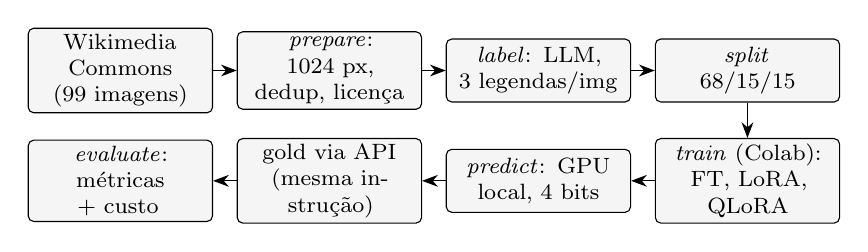
\begin{tikzpicture}[font=\footnotesize,
  box/.style={draw,rounded corners=2pt,align=center,minimum height=0.8cm,
              text width=2.2cm,fill=gray!8,inner sep=2pt},
  arr/.style={-{Stealth[length=2mm]}}, node distance=0.3cm]
\node[box] (a) {Wikimedia Commons\\(99 imagens)};
\node[box,right=of a] (b) {\textit{prepare}: 1024 px,\\dedup, licença};
\node[box,right=of b] (c) {\textit{label}: LLM,\\3 legendas/img};
\node[box,right=of c] (d) {\textit{split}\\68/15/15};
\node[box,below=0.45cm of d] (e) {\textit{train} (Colab):\\FT, LoRA, QLoRA};
\node[box,left=of e] (f) {\textit{predict}: GPU\\local, 4 bits};
\node[box,left=of f] (g) {gold via API\\(mesma instrução)};
\node[box,left=of g] (h) {\textit{evaluate}:\\métricas + custo};
\draw[arr] (a)--(b); \draw[arr] (b)--(c); \draw[arr] (c)--(d);
\draw[arr] (d)--(e); \draw[arr] (e)--(f); \draw[arr] (f)--(g);
\draw[arr] (g)--(h);
\end{tikzpicture}
\caption{Pipeline do experimento, da coleta à avaliação}
\label{fig:pipeline}
\end{figure}

As métricas de referência são BLEU \cite{papineni2002}, ROUGE-L
\cite{lin2004}, CIDEr \cite{vedantam2015} (texto em minúsculas, sem
pontuação, com acentos) e BERTScore \cite{zhang2020} com BERTimbau
\cite{souza2020}. A aderência imagem-texto usa CLIPScore e RefCLIPScore
\cite{hessel2021}, com CLIP ViT-B/32 \cite{radford2021} e codificador de
texto multilíngue \cite{reimers2020}. O custo inclui parâmetros treináveis,
VRAM, tempo de treino e de inferência.

\section{Resultados}

\subsection{Configuração do ambiente de experimentação}

São 99 imagens do Wikimedia Commons com licenças abertas, 7 delas do Porto de
Salvador; após excluir uma fora do domínio, ficaram 68 de treino, 15 de
validação e 15 de teste (semente 42). O treino rodou no Colab (NVIDIA L4,
22,5~GB, bf16): 3 épocas, lote efetivo 16, taxa de aprendizado
$2\times10^{-5}$ (pretrain), $10^{-5}$ (finetune, AdamW 8 bits) e $10^{-4}$
(LoRA/QLoRA, $r=16$, $\alpha=32$), imagens com lado de 448~px e
\textit{checkpoint} de menor perda de validação. A inferência rodou numa GPU
local de 4~GB, com as variantes em 4~bits e \textit{beam search} 3.

\begin{table}[ht]
\centering
\caption{Métricas no teste (N = 15; maior é melhor, exceto Palavras)}
\label{tab:metricas}
\footnotesize
\begin{tabular}{lccccccc}
\toprule
Variante & BLEU-4 & ROUGE-L & CIDEr & BERTScore & CLIPScore & RefCLIP & Palavras \\
\midrule
base     & 0,027 & 0,232 & 0,117 & 0,653 & \textbf{0,811} & \textbf{0,826} & 25,7 \\
pretrain & 0,086 & 0,304 & 0,249 & 0,703 & 0,723 & 0,798 & 20,9 \\
finetune & 0,067 & 0,307 & 0,290 & 0,711 & 0,701 & 0,775 & 20,4 \\
lora     & 0,142 & 0,359 & 0,507 & 0,737 & 0,665 & 0,771 & 20,9 \\
qlora    & \textbf{0,154} & \textbf{0,382} & \textbf{0,532} & \textbf{0,749} & 0,678 & 0,781 & 20,7 \\
\midrule
gold     & 0,225 & 0,440 & 0,870 & 0,790 & 0,706 & 0,806 & 21,8 \\
\bottomrule
\end{tabular}
\end{table}

\begin{table}[ht]
\centering
\caption{Custo de treino (Colab L4) e de inferência (GPU local, 4 bits)}
\label{tab:custo}
\footnotesize
\begin{tabular}{lrrrrr}
\toprule
Variante & Treináveis (M) & VRAM (GB) & Treino (min) & Perda val. & Inferência (s/img) \\
\midrule
base     & 0      & --   & --  & --    & 0,71 \\
pretrain & 100,7  & 8,01 & 1,7 & 2,153 & 0,72 \\
finetune & 1821,3 & 9,18 & 3,4 & 1,638 & 0,88 \\
lora     & 118,1  & 8,27 & 3,6 & 1,359 & 1,08 \\
qlora    & 118,1  & 8,20 & 2,7 & 1,394 & 1,24 \\
\bottomrule
\end{tabular}
\end{table}

\subsection{Experimento 1: adaptação ao domínio}

Compara \textit{base}, \textit{pretrain} e \textit{finetune}
(Tabela~\ref{tab:metricas}). Só ajustar o conector dobra o CIDEr (0,117 para
0,249), eleva o BERTScore em 0,05 e aproxima o tamanho das legendas do das
referências ($\sim$20,5 palavras); o fine-tuning completo acrescenta pouco
(CIDEr 0,290). O \textit{base} descreve cores, marcas e o céu (``gancho
vermelho com número 75'', ``caminhão Maersk''), o que a tarefa exclui.
\textbf{Resposta à QP1:} a adaptação melhora todas as métricas de
referência, e a maior parte do ganho vem do conector, isto é, de ajustar
como o LLM lê a imagem portuária.

\subsection{Experimento 2: eficiência em parâmetros}

Compara \textit{finetune}, \textit{lora} e \textit{qlora}
(Tabela~\ref{tab:custo}). Os adaptadores treinam 118~M parâmetros (6,5\% do
fine-tuning completo) e têm menor perda de validação (1,36 e 1,39 contra
1,64) e CIDEr 75--84\% maior. Com 68 imagens, ajustar todos os pesos
sobreajusta, e o posto baixo regulariza. Surgem termos do glossário
(\textit{reach stacker}, \textit{spreader}), mas também erros de grafia
(``contêiners'', ``portêinê'') penalizados pelas métricas lexicais. A
economia de VRAM do QLoRA foi pequena (8,20 contra 8,27~GB): num modelo de
2~B, o pico vem das ativações e do codificador de visão em 16~bits.
\textbf{Resposta à QP2:} sim, com 15$\times$ menos parâmetros e menos de
4 minutos de treino; a quantização não custou qualidade (a diferença entre
os dois está no ruído). O custo aparece na inferência: 1,24~s por imagem
contra 0,71~s do \textit{base}, por causa dos adaptadores não fundidos.

\subsection{Experimento 3: distância para o modelo grande}

O \textit{qlora} atinge 87\% do ROUGE-L, 95\% do BERTScore e 61\% do CIDEr
do \textit{gold}, que recebeu o mesmo glossário do rotulador e por isso tem
vantagem de vocabulário. O CLIPScore inverte a ordem: o \textit{base} tem o
maior valor (0,81), acima do \textit{gold} (0,71), pois o CLIP premia
atributos salientes proibidos pela especificação (cor, marcas, céu) e
conhece pouco o jargão em português, padrão próximo ao observado por
\citeasnoun{bromonschenkel2026}. \textbf{Resposta à QP3:} a distância
para o VLM grande é nítida no CIDEr e pequena nas métricas semânticas; as
métricas sem referência discordam das de referência e, aqui, medem
aderência visual genérica, não aderência à tarefa.

\section{Discussões e Ética}

As métricas medem a proximidade ao estilo do rotulador, um LLM sem revisão
humana, cujos erros são herdados pelo treino e pelo gabarito. O conjunto é
pequeno (15 imagens de teste, CIDEr instável), majoritariamente de portos
estrangeiros, com uma execução por variante; o Qwen pode ter visto imagens
do Commons no pré-treino, o \textit{gold} Flash baixa o teto e a inferência
quantizada pode subestimar as variantes. Quanto à ética, todas as imagens
têm licença aberta, com autoria registrada imagem a imagem. Trabalhadores
aparecem em algumas cenas; a especificação proíbe nomes e textos legíveis,
mas o \textit{pipeline} poderia ser reaproveitado para vigilância de
trabalhadores, uso que não endossamos. Um SLM local evita enviar imagens
operacionais a terceiros, mas legendas automáticas não substituem a inspeção humana em decisões de segurança.

\section{Conclusões e Trabalhos Futuros}

Um VLM de 2~B parâmetros, adaptado com 68 imagens e menos de 4 minutos de GPU
por variante, passou de legendas genéricas para legendas técnicas em
português, com LoRA e QLoRA à frente do fine-tuning completo e próximos de
um VLM grande nas métricas semânticas; o CLIPScore, sozinho, não serve para
avaliar legendas com especificação técnica. Como trabalhos futuros: ampliar
o conjunto para 300 imagens ou mais, com mais fotos do Porto de Salvador;
revisão humana do teste por especialistas portuários; várias sementes de
treino; e uma linha \textit{base} com o glossário no \textit{prompt}, para
separar o ganho de treino do ganho de instrução.

% Referencias no formato SBC (autor-ano). Rotulo entre colchetes = texto da citacao.
\begin{thebibliography}{99}

\bibitem[Alencar et al. 2024]{alencar2024}
Alencar, R.~S., Castañeda, W.~A.~C. and Amadeus, M. (2024).
\newblock Image captioning for Brazilian Portuguese using GRIT model.
\newblock {\em arXiv preprint arXiv:2402.05106}.

\bibitem[Bromonschenkel et al. 2026]{bromonschenkel2026}
Bromonschenkel, G., Koerich, A.~L., Paixão, T.~M. and de Oliveira, H.~T.~A. (2026).
\newblock Brazilian Portuguese image captioning with transformers: A study on cross-native-translated dataset.
\newblock {\em Journal of the Brazilian Computer Society}, 32(1):663--676.

\bibitem[Dettmers et al. 2023]{dettmers2023}
Dettmers, T., Pagnoni, A., Holtzman, A. and Zettlemoyer, L. (2023).
\newblock QLoRA: Efficient finetuning of quantized LLMs.
\newblock In {\em Advances in Neural Information Processing Systems (NeurIPS)}, volume~36.

\bibitem[Gemini Team 2023]{gemini2023}
Gemini Team, Google (2023).
\newblock Gemini: A family of highly capable multimodal models.
\newblock {\em arXiv preprint arXiv:2312.11805}.

\bibitem[Gondim et al. 2025]{gondim2025}
Gondim, J., Claro, D.~B. and Souza, M. (2025).
\newblock A bilingual analysis of multi-head attention mechanism for image captioning based on morphosyntactic information.
\newblock {\em Journal of the Brazilian Computer Society}, 31(1):1063--1076.

\bibitem[Heilig and Vo{\ss} 2017]{heilig2017}
Heilig, L. and Vo{\ss}, S. (2017).
\newblock Information systems in seaports: a categorization and overview.
\newblock {\em Information Technology and Management}, 18(3):179--201.

\bibitem[Hessel et al. 2021]{hessel2021}
Hessel, J., Holtzman, A., Forbes, M., Le~Bras, R. and Choi, Y. (2021).
\newblock CLIPScore: A reference-free evaluation metric for image captioning.
\newblock In {\em Proceedings of EMNLP}, pages 7514--7528.

\bibitem[Hu et al. 2022]{hu2022}
Hu, E.~J., Shen, Y., Wallis, P., Allen-Zhu, Z., Li, Y., Wang, S., Wang, L. and Chen, W. (2022).
\newblock LoRA: Low-rank adaptation of large language models.
\newblock In {\em International Conference on Learning Representations (ICLR)}.

\bibitem[Klar et al. 2023]{klar2023}
Klar, R., Fredriksson, A. and Angelakis, V. (2023).
\newblock Digital twins for ports: Derived from smart city and supply chain twinning experience.
\newblock {\em IEEE Access}, 11.

\bibitem[Lin 2004]{lin2004}
Lin, C.-Y. (2004).
\newblock ROUGE: A package for automatic evaluation of summaries.
\newblock In {\em Text Summarization Branches Out (ACL Workshop)}, pages 74--81.

\bibitem[Liu et al. 2023]{liu2023}
Liu, H., Li, C., Wu, Q. and Lee, Y.~J. (2023).
\newblock Visual instruction tuning.
\newblock In {\em Advances in Neural Information Processing Systems (NeurIPS)}, volume~36.

\bibitem[Lu et al. 2018]{lu2018}
Lu, X., Wang, B., Zheng, X. and Li, X. (2018).
\newblock Exploring models and data for remote sensing image caption generation.
\newblock {\em IEEE Transactions on Geoscience and Remote Sensing}, 56(4):2183--2195.

\bibitem[Molavi et al. 2020]{molavi2020}
Molavi, A., Lim, G.~J. and Race, B. (2020).
\newblock A framework for building a smart port and smart port index.
\newblock {\em International Journal of Sustainable Transportation}, 14(9):686--700.

\bibitem[Papineni et al. 2002]{papineni2002}
Papineni, K., Roukos, S., Ward, T. and Zhu, W.-J. (2002).
\newblock BLEU: a method for automatic evaluation of machine translation.
\newblock In {\em Proceedings of ACL}, pages 311--318.

\bibitem[Qwen Team 2025]{qwen3vl}
Qwen Team (2025).
\newblock Qwen3-VL-2B-Instruct.
\newblock Model card. \url{https://huggingface.co/Qwen/Qwen3-VL-2B-Instruct}.

\bibitem[Radford et al. 2021]{radford2021}
Radford, A., Kim, J.~W., Hallacy, C., Ramesh, A., Goh, G., Agarwal, S. et al. (2021).
\newblock Learning transferable visual models from natural language supervision.
\newblock In {\em Proceedings of ICML}, pages 8748--8763.

\bibitem[Reimers and Gurevych 2020]{reimers2020}
Reimers, N. and Gurevych, I. (2020).
\newblock Making monolingual sentence embeddings multilingual using knowledge distillation.
\newblock In {\em Proceedings of EMNLP}, pages 4512--4525.

\bibitem[Santos et al. 2022]{santos2022}
dos Santos, G.~O., Colombini, E.~L. and Avila, S. (2022).
\newblock \#PraCegoVer: A large dataset for image captioning in Portuguese.
\newblock {\em Data}, 7(2):13.

\bibitem[Shao et al. 2018]{shao2018}
Shao, Z., Wu, W., Wang, Z., Du, W. and Li, C. (2018).
\newblock SeaShips: A large-scale precisely annotated dataset for ship detection.
\newblock {\em IEEE Transactions on Multimedia}, 20(10):2593--2604.

\bibitem[Souza et al. 2020]{souza2020}
Souza, F., Nogueira, R. and Lotufo, R. (2020).
\newblock BERTimbau: Pretrained BERT models for Brazilian Portuguese.
\newblock In {\em Brazilian Conference on Intelligent Systems (BRACIS)}, pages 403--417. Springer.

\bibitem[Vedantam et al. 2015]{vedantam2015}
Vedantam, R., Zitnick, C.~L. and Parikh, D. (2015).
\newblock CIDEr: Consensus-based image description evaluation.
\newblock In {\em Proceedings of CVPR}, pages 4566--4575.

\bibitem[Vinyals et al. 2015]{vinyals2015}
Vinyals, O., Toshev, A., Bengio, S. and Erhan, D. (2015).
\newblock Show and tell: A neural image caption generator.
\newblock In {\em Proceedings of CVPR}, pages 3156--3164.

\bibitem[Xu et al. 2015]{xu2015}
Xu, K., Ba, J., Kiros, R., Cho, K., Courville, A., Salakhutdinov, R., Zemel, R. and Bengio, Y. (2015).
\newblock Show, attend and tell: Neural image caption generation with visual attention.
\newblock In {\em Proceedings of ICML}, pages 2048--2057.

\bibitem[Yang et al. 2018]{yang2018}
Yang, Y., Zhong, M., Yao, H., Yu, F., Fu, X. and Postolache, O. (2018).
\newblock Internet of things for smart ports: Technologies and challenges.
\newblock {\em IEEE Instrumentation \& Measurement Magazine}, 21(1):34--43.

\bibitem[Zhang et al. 2020]{zhang2020}
Zhang, T., Kishore, V., Wu, F., Weinberger, K.~Q. and Artzi, Y. (2020).
\newblock BERTScore: Evaluating text generation with BERT.
\newblock In {\em International Conference on Learning Representations (ICLR)}.

\end{thebibliography}


\end{document}
